%\documentclass[handout]{beamer}
%\documentclass[handout,10pt,slidestop,mathserif]{beamer}
%\usepackage{pgfpages}
%\pgfpagesuselayout{2 on 1}
\documentclass[10pt,slidestop,mathserif,c]{beamer}
\usetheme{Madrid}
\usecolortheme{seahorse}

\usepackage{tabularx}
\usepackage{verbatim}
\usepackage{graphics}
\usepackage{graphicx}
\usepackage{Sweave}
\usepackage{moreverb}
\usepackage{pgf}
\usepackage{tikz}

\newcommand{\putat}[3]{\begin{picture}(0,0)(0,0)\put(#1,#2){#3}\end{picture}}
  
\newenvironment{changemargin}[2]{%
  \begin{list}{}{%
    \setlength{\topsep}{0pt}%
    \setlength{\leftmargin}{#1}%
    \setlength{\rightmargin}{#2}%
    \setlength{\listparindent}{\parindent}%
    \setlength{\itemindent}{\parindent}%
    \setlength{\parsep}{\parskip}%
  }%
  \item[]}{\end{list}}

%% Define a new 'leo' style for the package that will use a smaller font.
\makeatletter
\def\url@leostyle{%
  \@ifundefined{selectfont}{\def\UrlFont{\sf}}{\def\UrlFont{\tiny\ttfamily}}}
\makeatother

\title[makeR Package]{Using the \texttt{makeR} Package for Managing Document Building and Versioning}
\subtitle{}
\author[Jason Bryer]{Jason M. Bryer}
\institute[jbryer.github.com]{University at Albany\\Excelsior College\\\url{jbryer.github.com/makeR}\\jason@bryer.org}
\date[useR! Conference - Jun 14, 2012]{June 14, 2012\\useR! Conference 2012\\Vanderbilt University\\Nashville, TN}

\begin{document}



\frame{\titlepage}
\frame{\frametitle{Agenda}\tableofcontents[hideallsubsections]}

\section{Overview}

\begin{frame}[fragile]
	\frametitle{Motivation}
	\begin{itemize}
	\item Need to create reports on a regular bases (i.e. montly, quarterly, yearly).
	\item The only difference from report-to-report tend to be date ranges and other easily abstracted data elements.
	\end{itemize}
	\pause
	There are tools and solutions such as:
	\begin{itemize}
	\item GNU make
	\item Batch files
	\item Java Ant
	\end{itemize}
	
	\pause
	However, there isn't a good solution implemented purely in R.
	
	\pause
	\ \\ \ \\
	And, since it took considerble effort to get my team to use R, introducing another program wasn't really an option!
\end{frame}

\begin{frame}[fragile]
	\frametitle{Goals and Workflow}
	The requirements include:
	\begin{itemize}
		\item Be implemented purely in R.
		\item Work on multiple platforms (i.e. Windows, Linux, and Mac).
		\item Maintain a history of ``released" versions.
	\end{itemize}
	\pause
	The workflow:
	\begin{itemize}[<+-| alert@+>]
		\item Define the project (once, subsequent sessions will restore state from an XML file)
		\item Define a new version (with the appropriate variables)
		\item Build
		\item Release
	\end{itemize}
\end{frame}

\begin{frame}[fragile,containsverbatim]
	\frametitle{makeR Package}
\begin{Schunk}
\begin{Sinput}
> ls('package:makeR')
\end{Sinput}
\begin{Soutput}
 [1] "builder.cacheSweave" "builder.knitr"      
 [3] "builder.rnw"         "builder.rnw.native" 
 [5] "builder.tex"         "calendarHeat"       
 [7] "env2string"          "getDefaultBuilder"  
 [9] "getRSSFeed"          "isAutoOpen"         
[11] "isAutoSave"          "Project"            
[13] "setAutoOpen"         "setAutoSave"        
[15] "setDefaultBuilder"   "varEntryDialog"     
\end{Soutput}
\end{Schunk}
	\pause
	Demos
	\begin{itemize}
		\item \texttt{r-bloggers} This demo will create a new makeR project that will provide a summary of R-Bloggers
		\item \texttt{stocks} This demo will demostrate creating a custom builder that outputs PNG files.
		\item \texttt{makeR-knitr} This demo will use the knitr package for building.
	\end{itemize}
\end{frame}


\begin{frame}
	\frametitle{Package Structure}
	\begin{center}
		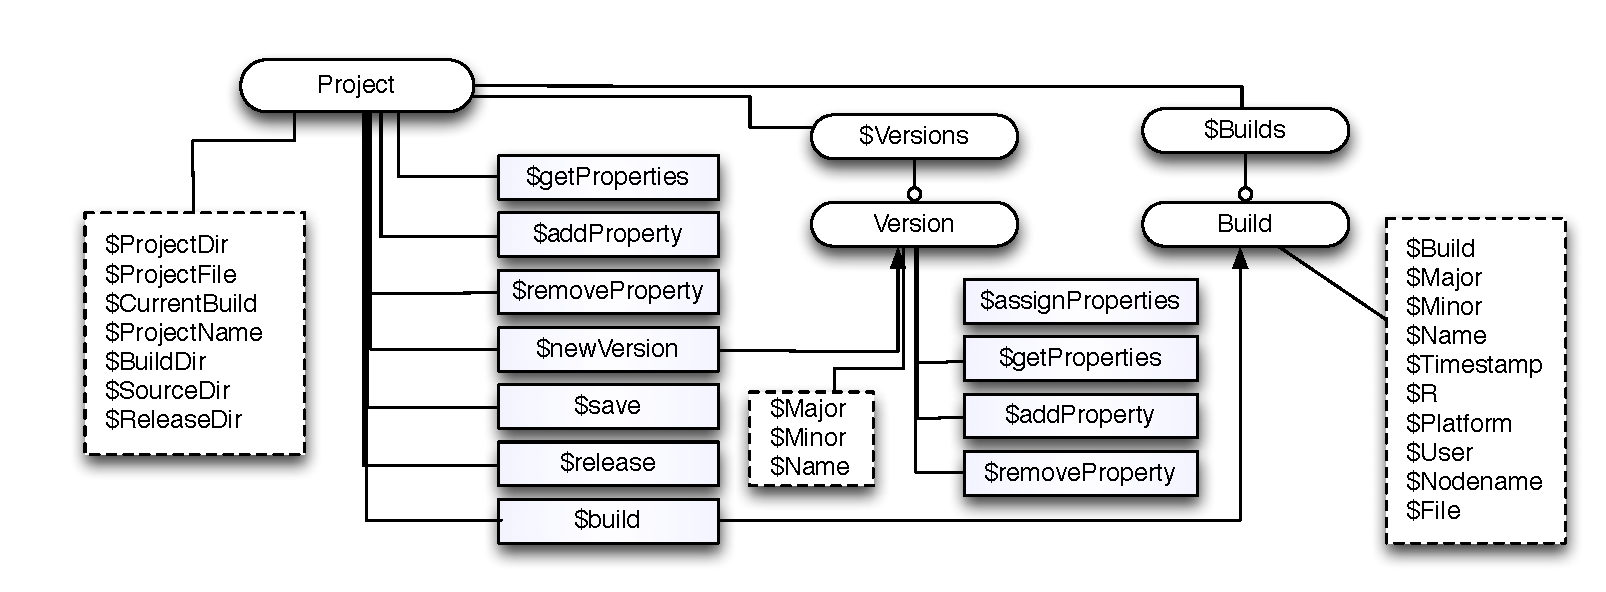
\includegraphics[width=\textwidth]{makeRClassDiagram.pdf}
	\end{center}
\end{frame}

\section{Sweave Example (R-Bloggers Demo)}
\begin{frame}[fragile,containsverbatim]
	\frametitle{R-Bloggers Example}
\begin{Schunk}
\begin{Sinput}
> myProject = Project(name="RBloggers", 
   			projectDir=projectDir, 
   			properties=list(
   				email=email, 
   				passwd=passwd))
\end{Sinput}
\end{Schunk}
\pause
\begin{Schunk}
\begin{Sinput}
> myProject$newVersion(name='2011-12', properties=list(
   			startDate='2011-12-01', endDate='2011-12-31'))
\end{Sinput}
\end{Schunk}
\pause
\begin{Schunk}
\begin{Sinput}
> myProject$build()
\end{Sinput}
\end{Schunk}
\pause
\begin{Schunk}
\begin{Sinput}
> myProject$release()
\end{Sinput}
\end{Schunk}
\end{frame}

\begin{frame}
	\frametitle{R-Bloggers Example Result}
	\begin{center}
		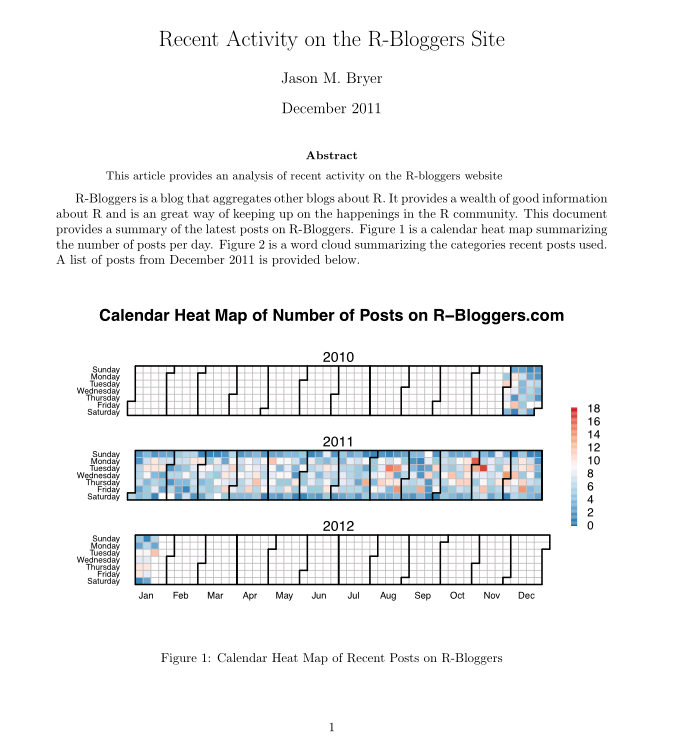
\includegraphics[width=.7\textwidth]{rbloggers.png}
	\end{center}
\end{frame}

\section{Extensibility (Stocks Demo)}

\begin{frame}[fragile,containsverbatim]
	\frametitle{Customer Builders}
	
\begin{Schunk}
\begin{Sinput}
> builder.png <- function(project, theenv, ...) {
   	sourceFile = ifelse(is.null(project$SourceFile), '.r$', 
   						project$SourceFile)
   	wd = eval(getwd(), envir=theenv)
   	files = list.files(path=wd, 
   					   pattern=sourceFile, 
   					   ignore.case=TRUE)
   	for(i in seq_len(length(files))) {
   		cat(paste("Executing ", files[i], "...", sep=''))
   		sys.source(files[i], envir=theenv)
   	}
   	return(list.files(path=wd, pattern=".png$", 
   					  ignore.case=TRUE))
   }
\end{Sinput}
\end{Schunk}
\end{frame}

\begin{frame}[fragile,containsverbatim]
	\frametitle{Customer Builders}
\begin{Schunk}
\begin{Sinput}
> stocksProject = Project(name="stocks", 
   projectDir=projectDir, properties=list(
   	src = "yahoo", stocks = c("GOOG",'AAPL','AMZN','MSFT','FB')))
\end{Sinput}
\end{Schunk}

\begin{Schunk}
\begin{Sinput}
> stocksProject$newVersion(name='2012-05', 
   		properties=list(month='2012-05'))
\end{Sinput}
\begin{Soutput}
Version 1.0
Name: 2012-05
Properties:
  month = 2012-05
\end{Soutput}
\end{Schunk}

\end{frame}

\begin{frame}[fragile,containsverbatim]
	\frametitle{Custom Builders (cont.)}
\begin{Schunk}
\begin{Sinput}
> stocksProject
\end{Sinput}
\begin{Soutput}
Project Directory: /Users/jbryer/R/makeR/demo/stocksDemo
Source Directory: source
Build Directory: build
Current build: 0
Properties:
  src = yahoo
  stocks = GOOG, AAPL, AMZN, MSFT, FB
There are currently 1 versions defined:
$`1`
Version 1.0
Name: 2012-05
Properties:
  month = 2012-05
\end{Soutput}
\end{Schunk}
\end{frame}

\begin{frame}[fragile,containsverbatim]
	\frametitle{Custom Builders (cont.)}
\begin{Schunk}
\begin{Sinput}
> stocksProject$build(builder=builder.png)
\end{Sinput}
\begin{Soutput}
Building verison 2012-05.0-1...
Setting global properties...
src = yahoo
stocks = GOOG, AAPL, AMZN, MSFT, FB
Setting version properties...
month  =  2012-05
Copying source files...
Building version 1.0-1
Saving build environment to build.1.0-1.Rda
\end{Soutput}
\end{Schunk}

\begin{Schunk}
\begin{Sinput}
> stocksProject$release(version='2012-05')
\end{Sinput}
\begin{Soutput}
Copying build/2012-05.0/2012-05.png to release/2012-05-2012-05.0.png
\end{Soutput}
\end{Schunk}
\end{frame}

\begin{frame}[fragile,containsverbatim]
	\frametitle{Stocks Example Result}
	\begin{center}
\includegraphics[width=.7\textwidth]{{/Users/jbryer/R/makeR/demo/stocksDemo/release/2012-05-2012-05.0}.png}
	\end{center}
\end{frame}

\section{Customizing makeR}
\begin{frame}[fragile,containsverbatim]
	\frametitle{Customizine makeR}
	
	\begin{itemize}[<+-| alert@+>]
		\item \texttt{getDefaultBuilder} \& \texttt{setDefaultBuilder} \\
		Returns and sets the default builder for the current R session.
		\item \texttt{getAutoOpen} \& \texttt{setAutoOpen} \\
		\texttt{makeR} will, by default, attempt to open the built or released file using the default application for the file type (e.g. PDF, TIFF, etc.)
		\item \texttt{getAutoSave} \& \texttt{setAutoSave} \\
		\texttt{makeR} saves project state in an XML file. If you wish to not save the XML file automatically, you can set this to FALSE. For example, you could save the project state to an RData file.
	\end{itemize}
\end{frame}

\section{Debugging Projects}
\begin{frame}[fragile,containsverbatim]
	\frametitle{Debegging}
\begin{Schunk}
\begin{Sinput}
> stocksProject$Versions[[1]]$assignProperties()
\end{Sinput}
\begin{Soutput}
Setting global properties...
src = yahoo
stocks = GOOG, AAPL, AMZN, MSFT, FB
Setting version properties...
month  =  2012-05
\end{Soutput}
\end{Schunk}
\end{frame}

\section{The XML File}
\begin{frame}[fragile,containsverbatim]
	\frametitle{The \texttt{makeR} XML File}
\begin{verbatim}
<?xml version="1.0"?>
<project name="stocks" buildDir="build" releaseDir="release" 
    sourceDir="source">
  <property name="src" type="character">
    <value>yahoo</value>
  </property>
  <property name="stocks" type="character">
    <value>GOOG</value>
    <value>AAPL</value>
    <value>AMZN</value>
    <value>MSFT</value>
  </property>
  ...
\end{verbatim}
\end{frame}

\begin{frame}[fragile,containsverbatim]
	\frametitle{The \texttt{makeR} XML File (cont.)}
\begin{verbatim}
  ...
  <versions>
    <version name="2011-12" major="1" minor="1">
      <property name="month" type="character">
        <value>2011-12</value>
      </property>
    </version>
  </versions>
  ...
\end{verbatim}
\end{frame}

\begin{frame}[fragile,containsverbatim]
	\frametitle{The \texttt{makeR} XML File (cont.)}
\begin{verbatim}
  ...
  <builds>
    <build major="1" minor="0" build="1" name="2011-12" 
        timestamp="Thu Jan 26 20:55:10 2012"
        R="R version 2.14.0 (2011-10-31)" 
        platform="x86_64-apple-darwin9.8.0"
      nodename="Jason-Bryers-MacBook-Air-2.local" user="jbryer">
      <file>2011-12.png</file>
    </build>
  </builds>
</project>
\end{verbatim}
\end{frame}

\begin{frame}
	\frametitle{Future Directions}
	\begin{itemize}
	\item Provide hooks into the release process. 
	\item Provide helper functions for scheduled runs.
	\item Allow properties to be assigned interactively at runtime instead of saved in the XML file (e.g. passwords).
	\item Builder for R Markdown.
	\end{itemize}
\end{frame}

\begin{frame}[c]
	\LARGE{Thank You}\\
	\normalsize
	Jason Bryer (jason@bryer.org)\\
	\url{http://jbryer.github.com}
\end{frame}

\begin{frame}[fragile,containsverbatim,shrink=5]
	\frametitle{Session Info}
\begin{Schunk}
\begin{Soutput}
R version 2.15.2 (2012-10-26)
Platform: x86_64-apple-darwin9.8.0/x86_64 (64-bit)

locale:
[1] en_US.UTF-8/en_US.UTF-8/en_US.UTF-8/C/en_US.UTF-8/en_US.UTF-8

attached base packages:
[1] tools     graphics  grDevices utils    
[5] datasets  stats     methods   base     

other attached packages:
[1] quantmod_0.3-17 TTR_0.21-1     
[3] xts_0.8-6       zoo_1.7-8      
[5] Defaults_1.1-1  makeR_1.0.2    
[7] XML_3.95-0.1    ggplot2_0.9.2.1

loaded via a namespace (and not attached):
 [1] colorspace_1.2-0   dichromat_1.2-4   
 [3] digest_0.5.2       grid_2.15.2       
 [5] gtable_0.1.1       labeling_0.1      
 [7] lattice_0.20-10    MASS_7.3-22       
 [9] memoise_0.1        munsell_0.4       
[11] plyr_1.7.1         proto_0.3-9.2     
[13] RColorBrewer_1.0-5 reshape2_1.2.1    
[15] scales_0.2.2       stringr_0.6.1     
\end{Soutput}
\end{Schunk}
\end{frame}

\end{document}
